% Template for ICIP-2015 paper; to be used with:
%          spconf.sty  - ICASSP/ICIP LaTeX style file, and
%          IEEEbib.bst - IEEE bibliography style file.
% --------------------------------------------------------------------------
\documentclass{article}

\usepackage{spconf,amsmath,graphicx}
\usepackage{caption}


%\textwidth=178mm  
%\textheight=229mm
%\marginparwidth=19mm 
%\topmargin=35mm


% Example definitions.
% --------------------
\def\x{{\mathbf x}}
\def\L{{\cal L}}

% Title.
% ------
\title { On Deep Convolutional networks for large scale image classification}
%
% Single address.
% ---------------
\name{Mahesh C., Student Member, IEEE, Madhu S. Nair, Member, IEEE}
\address{Department of Computer Science, University of Kerala, Kariavattom\\ Thiruvananthapuram-695581,
	Kerala, India.
}
%
% For example:
% ------------
%\address{School\\
%	Department\\
%	Address}
%
% Two addresses (uncomment and modify for two-address case).
% ----------------------------------------------------------
%\twoauthors
%  {A. Author-one, B. Author-two\sthanks{Thanks to XYZ agency for funding.}}
%	{School A-B\\
%	Department A-B\\
%	Address A-B}
%  {C. Author-three, D. Author-four\sthanks{The fourth author performed the work
%	while at ...}}
%	{School C-D\\
%	Department C-D\\
%	Address C-D}
%

\begin{document}
\topmargin=0mm 
%\ninept
%
\maketitle
%
\begin{abstract}
Image classification is an essential to the field of computer vision  based systems and recent research in this area explores better feature extraction, feature coding, and classification.  The purpose of this paper is to review the application of supervised  deep convolution networks in this field. Numerous techniques have been reported to improve the performance of the convolution networks. Experimental analysis shows that with a large amount of labeled data, convolution networks can learn very complex functions such as image classification. 



\end{abstract}
%
\begin{keywords}
convolution networks, deep learning, neural networks.
\end{keywords}
%
\section{Introduction}
\label{sec:intro}
The performance of an  image  classification system mainly depends on the  extraction and  representation of features.  Feature representation methods like Haralick texture features \cite{Haralick1973} got attention from the research community from the earlier days of  image classification. However, to develop features that are invariant to position, rotation, scaling, and distortion, researchers had  to  explore the visual perception of primates. This research  led to  the development of many models such as convolutional neural networks\cite{LeCun1998} and  Kohonen map\cite{kohonen1982self}. 
As a result, many successful image classification systems are  implemented with better accuracy \cite{lecun-89e}.

Early in that stage, method like the convolutional network is limited by the  availability of labeled  data and computing infrastructure. Researchers are trying to overcome  this problem by many other non-parametric models such as SVM and KNN. But these methods couldn't give a high accuracy result  on any of the large-scale classification problem  and limited by the preprocessing technique.  However, in the recent years, the development of  High Performance Computing (HPC) architecture such as General Purpose Graphical Processing Units (GPGPU)  accelerated the research in this field. Large scale image  dataset such as ImageNet \cite{imagenet}  with  millions of labeled samples is also accessible to the research community. These changes in data and computing, put back the convolution network with millions of parameters in track. 


\section{Multi-stage Hubel-Wiesel architecture}
In 1962, Hubel DH and Wiesel TN \cite{Hubel1962}, \cite{Hubel1965a}  studied visual cortex of anesthetized cats  with   spots of white light of various shapes. Cells in the visual system are classified    into  simple, complex and hypercomplex. Simple cells are influenced  by the arrangement of  excitatory and inhibitory regions of the receptive field as well as the position of the stimulus. This cell receives input from cells of the lateral geniculate nucleus (LGN), which is connected to the retina. However, the complex cells will respond to  an appropriately  oriented stimulus regardless of the cell position in the receptive field. Complex cells are activated by edge, dark bar, slit and mixed stimuli. Hypercomplex cells are activated by edge, single-stopped (corner), double-stopped (tongue), slit (double-stopped) and dark bar (double-stopped).

\par In the visual cortex, perception cells are in the  order, simple$\Longrightarrow$complex$\Longrightarrow$lower-order-hypercomplex$\Longrightarrow$higher-order-hypercomplex. Activation of  a lower stage is  influenced by  the position of the input patterns, and  higher stages are  position-invariant. There are several  contradictory to this structure, but no one   completely deny this hierarchical model.
\par Inspired by this work, Fukushima, K \cite{Stark1980} proposed a neural network model for pattern recognition called neocognitron.
In neocognitron, cells are arranged in  a number of  cascaded structure. Each  structure $U$ include a  simple cell layer $U_s$ and a complex cell layer $U_c$. This network is not affected by change in position or small distortion in the shape of patterns.  It is also capable of doing self-organization based on an unsupervised competitive learning algorithm \cite{Fukushima1982} in the first two layers and classification based on  supervised learning in the output layer.
\begin{figure}[ht]
 \centering
 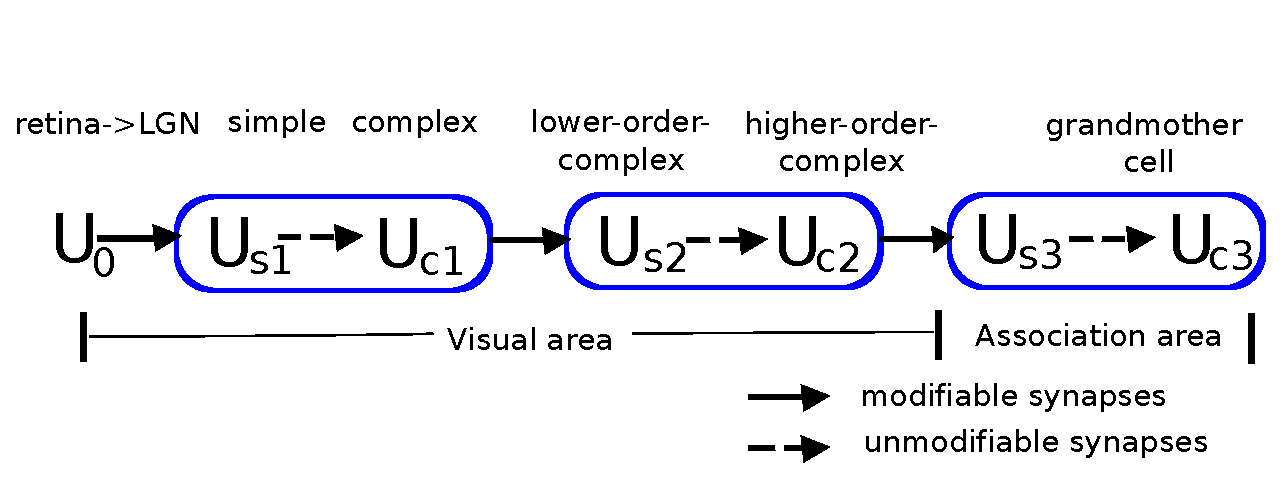
\includegraphics[width=8cm]{Figures/neocognitron.eps}
 \captionsetup{justification=centering,belowskip=0pt,aboveskip=0pt}
\caption{Neocognitron}
\label{neo}
\end{figure}
\section{Convolutional Networks}
\par Neocognitron was improved by  Yann LeCun \cite{lecun-86}, \cite{lecun-89e}, using backpropagation algorithm  to train the entire system. It uses local receptive fields, share weights and  sub-sampling to achieve  shift, position and distortion invariance. A typical Convolutional Network called  LeNet-5 was proposed by   Yann LeCun et al. \cite{LeCun1998}  for document recognition. Using \allowbreak local receptive fields, network can extract elementary visual features such as edges, end points and corners. These features will be combined to obtain high order features in the following layers. Elementary feature detectors with identical weights can be useful in different parts of the image. So the units with  the same set of weights are arranged in plane, and output from  the units of a plane is called  a feature map. Units in  a feature map perform the same operation on different parts of the same image. A convolution layer is composed of the set of feature maps with differently weighed units. In the implementation, a unit in the feature map scans the image and store the states in the feature map. This operation is equivalent to convolution with a kernel composed of a  set of weights and image. 

\par
A typical convolutional  network is composed of multiple stages with a filter bank layer, a non-linearity layer and a feature pooling layer \cite{lecun2010convolutional} followed by a classification network.\\
\begin{figure}[ht]

 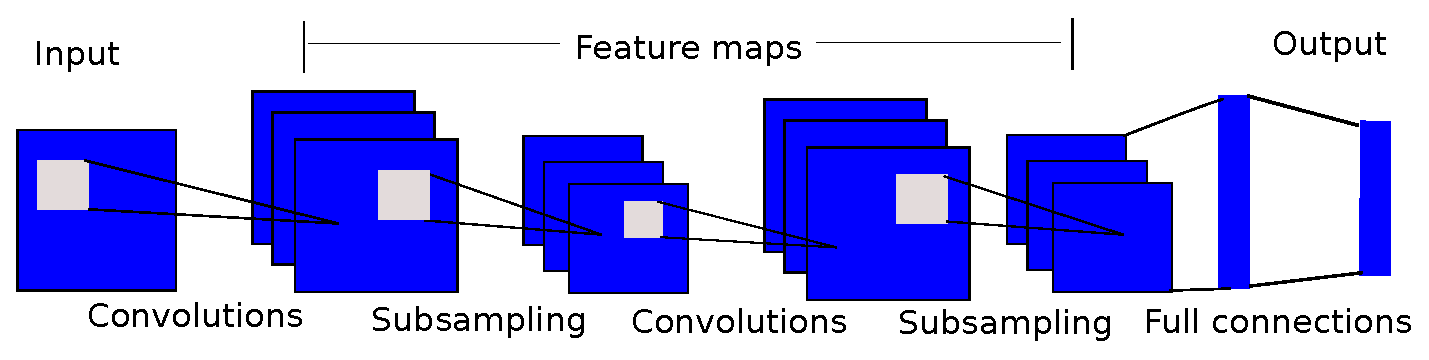
\includegraphics[width=7cm]{Figures/convent.eps}
\caption{A typical convolutional network architecture }
\label{net}
\end{figure}
\emph{Filter Bank Layer:} This layer computes $y_{j}$ the convolution between an input feature map   $x_i$ and trainable filter kernel $k_{ij}$ 
 ie. $y_j=b_j+\sum_i {k_{ij}*x_i}$, where $b_j$ is a trainable bias, $i$ and $j$ are  array indices, and $*$ is the convolution operator.\\
\emph{Non-Linearity Layer:} This layer applies a non-linearity function such as $tanh(x)$ or $(1+e^{-x})^{-1}$ to unit output. But to reduce training time with gradient descent, new implementations uses the function $max(0,x)$. Units with this non-linearity is called Rectified Linear Units (ReLUs) \cite{Nair2010}.\\
\emph{Feature Pooling Layer:} It  reduces the dimension of  feature map by applying the techniques like averaging or max-pooling.


% -------------------------------------------------------------------------
\begin{figure}[t]

\begin{minipage}[b]{.48\linewidth}
  \centering
  \centerline{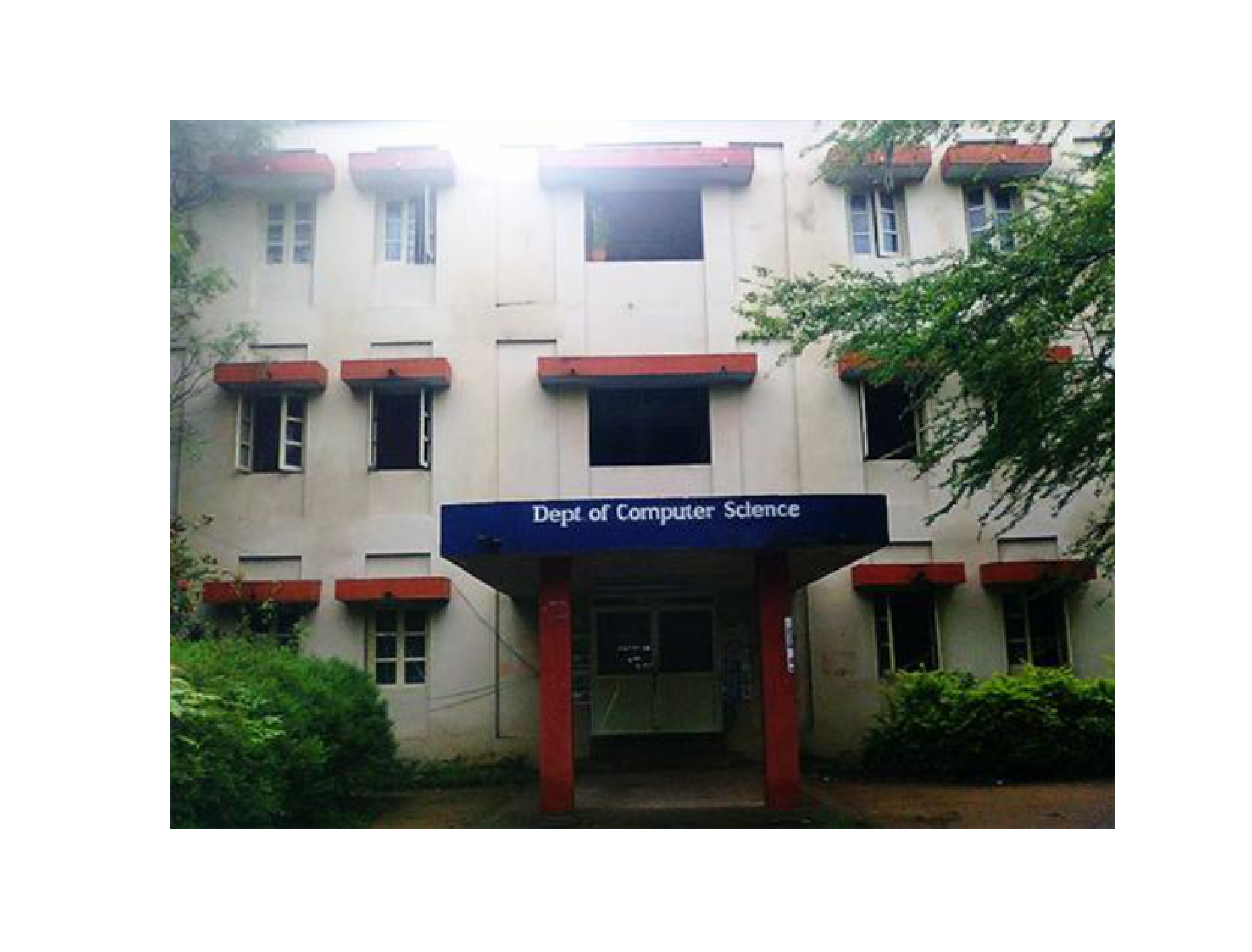
\includegraphics[width=3.8cm]{Figures/org}}
%  \vspace{2.0cm}
  \centerline{Input image}\medskip
\end{minipage}
%
\begin{minipage}[b]{.48\linewidth}
  \centering
  \centerline{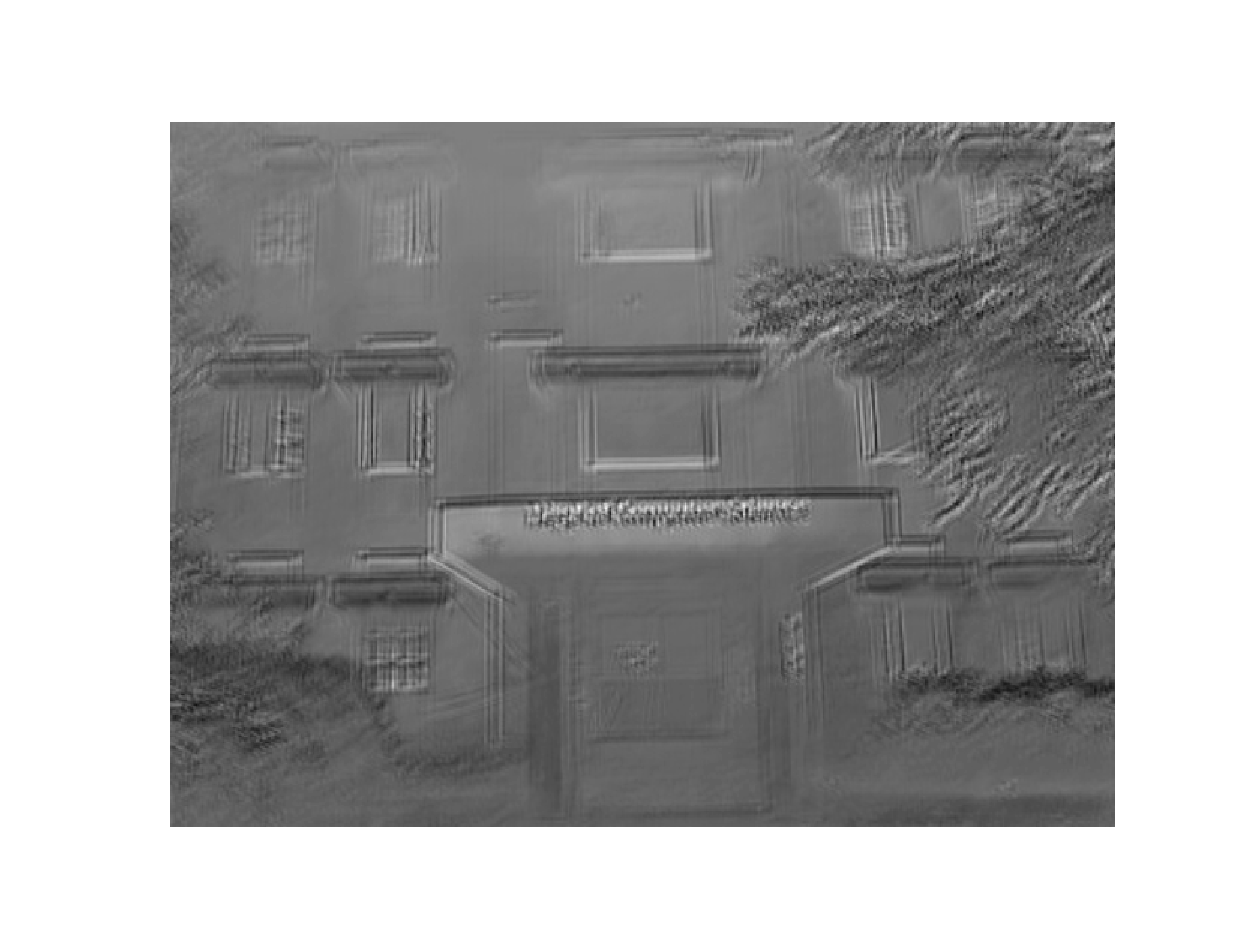
\includegraphics[width=3.8cm]{Figures/first}}
%  \vspace{1.5cm}
  \centerline{Output - first component }\medskip
\end{minipage}
\hfill
\begin{minipage}[b]{0.48\linewidth}
  \centering
  \centerline{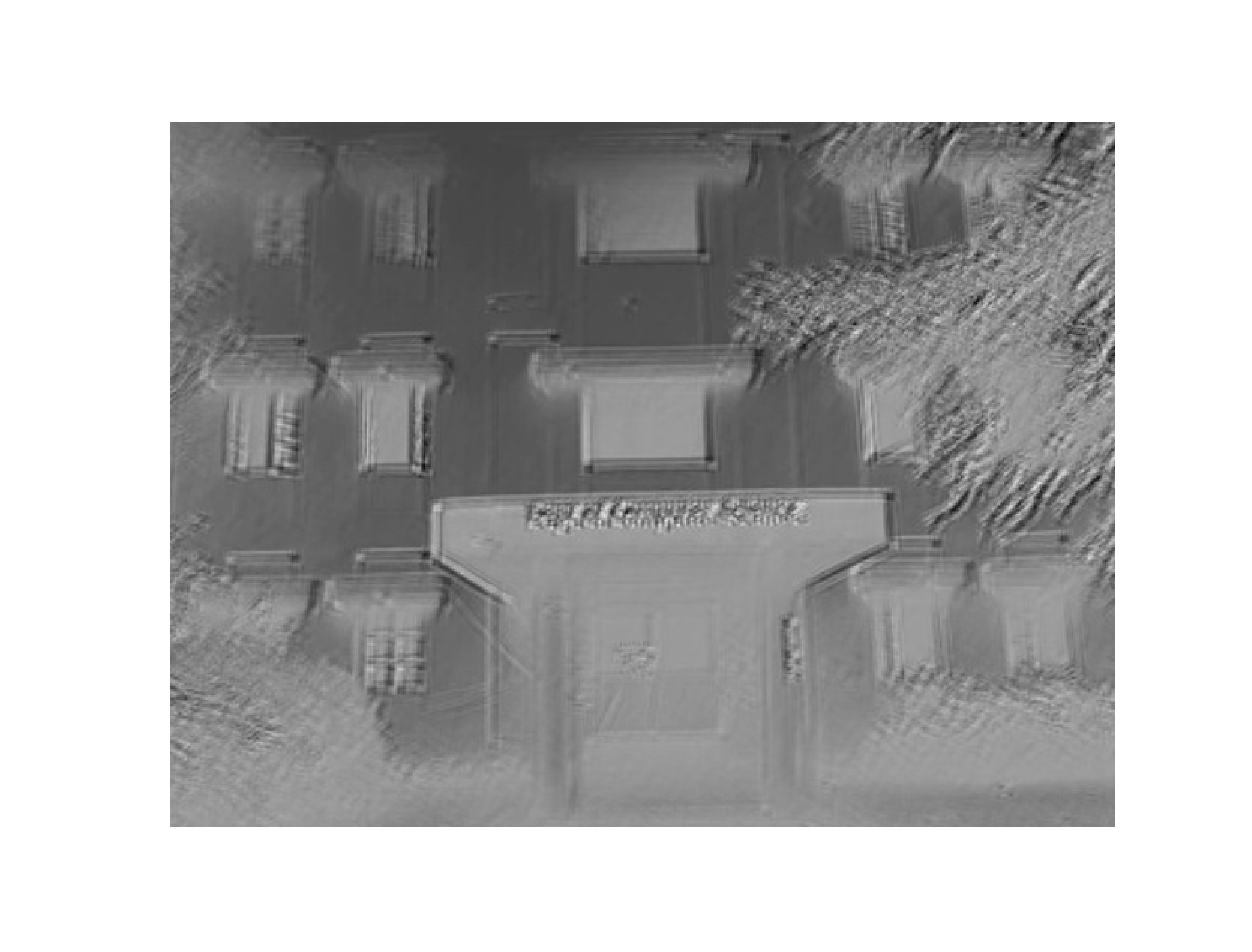
\includegraphics[width=3.8cm]{Figures/second}}
%  \vspace{1.5cm}
  \centerline{Output - second component}\medskip
\end{minipage}
%
\begin{minipage}[b]{0.48\linewidth}
  \centering
  \centerline{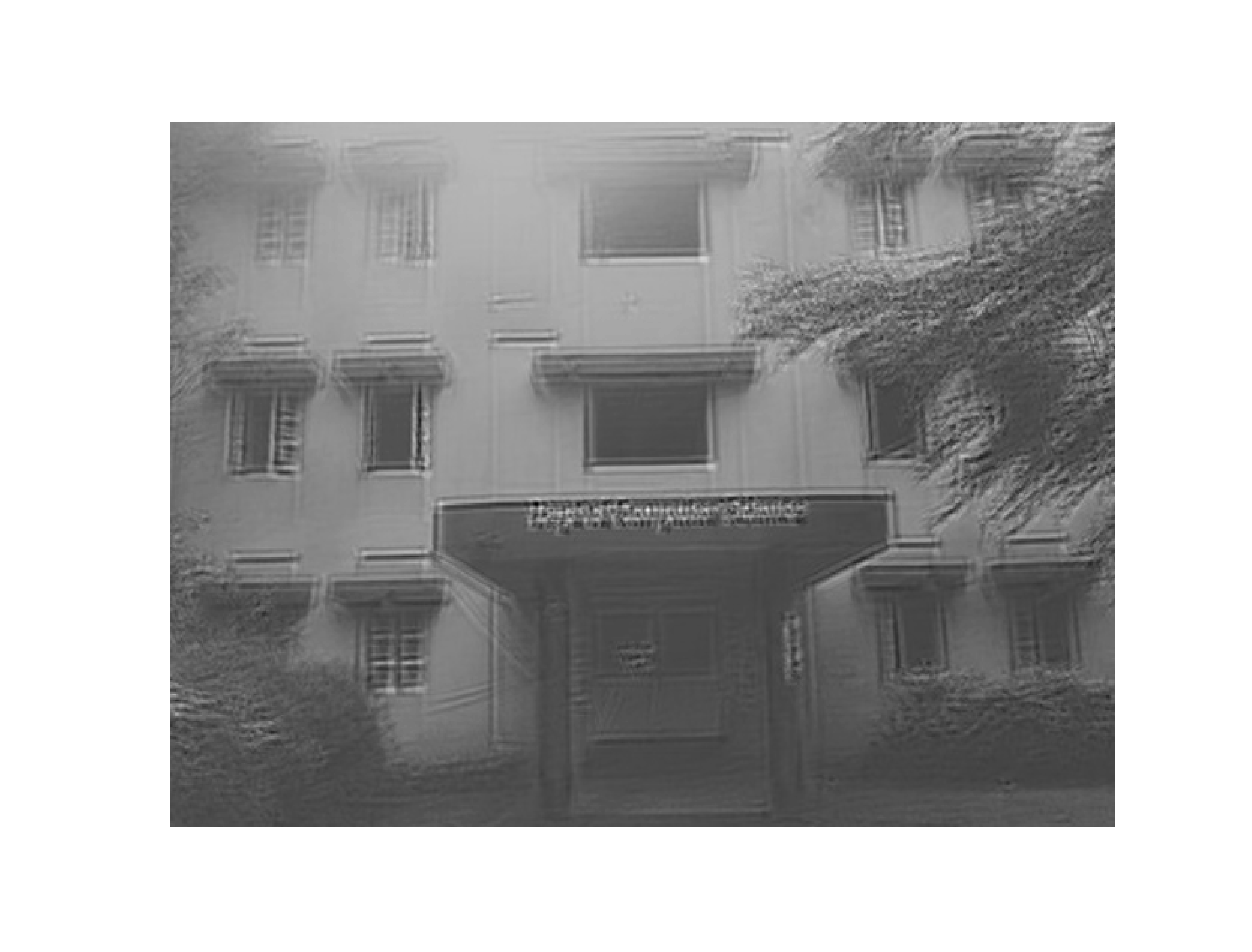
\includegraphics[width=3.8cm]{Figures/third}}
%  \vspace{1.5cm}
  \centerline{Output - third component}\medskip
\end{minipage}
%
\caption{Output of a randomly initialized convolution filter.
}
\label{fig:res}
%
\end{figure}




But this architecture was limited by the availability of computing power and  sample data sets. 
%2012

\section {Deep convolutional networks}
In the last few years, convolutional networks shows a significant performance improvement in many small scale image classification on data sets  such as MNIST \cite{Ciresan:2012g}, CIFAR-10, CIFAR-100, SVHN \cite{lee2014deeply}, and STL-10 \cite{deepfwd}. Krizhevsky, et al. \cite{Krizhevsky2012a} proposed a network  of 60 million parameters and 650,000 neurons, with five convolutional layers followed by max-pooling layers and three fully-connected layers. Data set used in this experiment was a subset of ImageNet dataset, used in the competition ImageNet Large-Scale Visual Recognition Challenge (ILSVRC) \cite{imagenet} and reported an error rate of 15.3\%. ILSVRC data set includes 1.2 million images that contain 1,000 categories. This network uses rectifier  as the function in neurons.  Even if it shows improvement in speed, this  ill-conditioned parameterization must be studied further to understand the effect in very large networks.


%2013

\subsection{Network in Network }
Inspired by the work of Ian J. Goodfellow et al..\cite{Goodfellow2013} on max out networks,  Min Lin et al. \cite{Lin2013} introduced a micro-network in each convolution layer so that it will compute more abstract features.This network gave a state-of-the-art performance in  ILSVRC 2013 competition with an error rate of 12.95\%.They used NVIDIA TITAN GPU to train the network. Using multilayer perceptron instead of voting to approximate convex functions of each  local patches may result in a good accuracy; but this is equivalent to moving linear separability problem into another hyperspace. So, if the input is in high frequency, this will end up in modeling large number of hidden layers and make the network structure more dependent on the problem. It will diverge the idea of the convolution network from \emph{learn anything} to a \emph{local search}.

\subsection{Visualizing Convolutional Networks}

Matthew D. Zeiler and Rob Fergus \cite{Zeiler2013} presented a method to visualize the function of intermediate feature layers of convolutional networks and used it as a diagnostic tool to improve  the model proposed by Krizhevsky et al. \cite{Krizhevsky2012a}. This method helped  them  to understand  the activation in the feature maps with respect to the input patterns. It shows that Krizhevsky et al.'s architecture does not have  enough mid frequency coverage in the first layer filters and causes aliasing artifacts by large stride in the first layer convolutions. Authors solved this problem by decreasing filter size to $7\times7$ and reducing stride to 2. This implementation won the  ILSVRC 2013 competition with an error rate of 11.74\%. These  techniques might be more useful if it can relate to any of the learning formulations instead of vague approximations of a non-invertible function.


%2014

\subsection{Spatial Pyramid Pooling in Deep Convolutional Networks}
Instead of using fixed input size in convolutional networks, Kaiming He et al. \cite{He2014} suggested  the use of a spooling strategy called  Spatial Pyramid Pooling (SPP) \cite{Grauman2005} \cite{1641019} to avoid cropping or warping of images. It introduced a new layer on top of the convolution layer and performed aggregation  based on Bag-of-Words (BoW) model. However, the classical backpropagation training methods expect layers to have a fixed   size.  This problem can be solved by using two fixed size networks with shared parameters and switch the network on alternate epochs. Network was trained using a single GeForce GTX Titan GPU with a starting  learning rate of 0.01 and achieved  a less  error rate of 8.06\% on  ILSVRC 2014 data set. 
\par 
This implementation improves the performance of baseline architectures including ZF-5 \cite{Zeiler2013}, Convnet \cite{Krizhevsky2012a} and Overfeat-5/7. Even if  the accuracy of convolutional networks will improve on multi-size training, multi-level pooling, and full-image representations, all these methods will increase both time and space complexity of the system.
%




\subsection{Going deeper with convolutions }
Christian Szegedy et al. \cite{Szegedy} proposed a network named GoogLeNet with receptive field (input layer) of size $244\times244$ with the number of layers around 100. Network is trained using asynchronous stochastic gradient descent with 0.9 momentum and fixed learning rate schedule based on the number of epochs. Learning procedure took advantage of  model and data-parallelism in a CPU-based cluster environment. This network gave an error rate of  6.67\%  on  ILSVRC 2014 data set. The experimental analysis shows that use of existing dense  blocks to  build the sparse structure can improve the  performance of convolutional networks. Even if higher depth will increase the accuracy, this system will end up with implementing large number of hidden layers to increase accuracy for a high frequency input. 


\section{VERY DEEP CONVOLUTIONAL NETWORKS }
Karen Simonyan and Andrew Zisserman \cite{Arge2015} evaluated the effect of network depth in image classification using very small convolution filters. Their deep network architecture comprised of fixed  size input layers, a stack of convolution layers, three Fully-Connected (FC) layers and  5 max-pooling layers for spatial pooling  over a $2 \times 2$ pixel window with stride 2. Hidden layers are modeled using Rectified Linear Units (ReLU) \cite{Nair2010}. On the hardware side, it uses a multi-GPU system with NVIDIA Titan Black GPUs. Network is trained using multinomial logistic regression  based on backpropagation with momentum of 0.9 and  batch size  256.
\par
It has been observed that greater depth with small convolution filters and  initialization of certain layers will cause the learning process to converge in less number of epochs and gain significant improvement in accuracy. This model of the convolution network does not differ from the classical architecture proposed by LeCun et al. \cite{LeCun1998}. This implementation results in a significant improvement in accuracy with  an error rate of 6.8\% in ILSVRC 2014 of ImageNet.

\begin{subsection}{Scaling up Image Classification}
The latest attempt in image classification with an error rate of 5.98\% in ImageNet data set is reported by Ren Wu et al. \cite{Wu2015} of Baidu research. They developed an end to end deep learning  system named Deep Image. It uses a highly optimized parallel algorithm to implement large deep neural network with augmented input data. The network is trained using Stochastic Gradient Descent algorithms (SGD) on a custom built high performance system comprised of 36 server nodes, each with 2 six-core Intel Xeon E5-2620 processors and 4 NVIDIA Tesla K40m GPUs. System  uses an InfiniBand  network for interconnections. Parallelism strategies used in this network are model-data parallelism and data parallelism. These methods have been proposed by Alex Krizhevsky \cite{Krizhevsky2014} and Omry Yadan et al. \cite{Yadan2013} for training convolutional neural networks with SGD on a  multiple GPU systems. However, it is not easy to extend the same strategies to multiple GPU clusters because of the communication overhead. The major objective is to minimize network data transfers and dynamic computation. So it uses butterfly synchronization and lazy update strategies to achieve data parallelism in the gradient computation. These approaches shows that model-data parallelism is better when number of GPUs is less than 16. %Implementation of Data parallelism in a large number of GPU cluster is better because of the constant communication requirements.
\par
Data augmentation techniques are used to increase the number of labeled images in the training set. This includes color casting, vignetting, lens distortion, rotation, flipping and cropping. But this data augmentation techniques  does not solve the major problems such as occlusion, presence or absence of structural components, and lighting conditions.
\centering
\begin{table*}[ht]
\captionsetup{justification=centering,belowskip=1pt,aboveskip=1pt}
\caption[]{ Comparative analysis of state-of-the-art deep convolutional network based image classification algorithms using ILSVRC dataset.}
 \begin{tabular}{ | p{2.7cm} | l | p{1.4cm} |p{1.1cm} |p{.8cm} |p{1.3cm} |p{1.1cm} |p{5cm}|}

    \hline
\textbf{Team}	&\textbf{Year}	&\textbf{Data Augmentation}	&\textbf{Scalable over network}	&\textbf{Time taken}	&\textbf{Hardware}	&\textbf{Error rate} &\textbf{Observations}
\\ 
\hline
Ren Wu et al. \cite{Wu2015}&2015&Aggressive&Yes&8.8 hours&Multi-GPU Cluster&5.98\%&Aggressive augmentation  will make the problem dependent on data set.\\
\hline
Karen Simonyan et al. \cite{Arge2015}&2014&Minimum&No&3 weeks&Multi-GPU&6.80\% &Effect of small convolution filter in low frequency domain need to be studied.\\
\hline
Christian Szegedy et al. \cite{Szegedy}&2014&Minimum&Yes&1 week&CPU Cluster&6.67\% &Inserting more layers will make system depend on the data set.\\
\hline
Kaiming He et al. \cite{He2014}&2014&Minimum&No&4 weeks	&Single GPU	&8.06\% &Good method, but higher time complexity.\\
\hline
Matthew D. Zeiler et al. \cite{Zeiler2013}&2013&Minimum&No&12 days&Single GPU&11.74\% & Visualizations are not possible in very deep network.\\
\hline
Min Lin et al. \cite{Lin2013}&2013&Minimum&No&12 days&Single GPU&12.95\% &Inserting more layers will over-fit the system.\\
\hline
Krizhevsky, et al.\cite{Krizhevsky2012a}&2012&Minimum&No&6 days	&Multi-GPU&15.30\%&Effect of rectifier must be studied further.\\
\hline

\end{tabular}
\label{table_cp}
\end{table*}
\par
 Major contribution of this work is the demonstration of tremendous computational power required to  achieve high accuracy in image classification.
It also shows that augmented multi-scale images can be combined to achieve less error rate in convolutional network in the context of the image classification. 
 \end{subsection}
 \section {Observations}
In recent years, the research community has reported several image classification algorithms based on deep convolutional network which gives less rate. A comparative analysis of recent futuristic deep convolutional networks is shown in Table \ref{table_cp}.
  Ren Wu et al. \cite{Wu2015} uses aggressive data argumentation and high computational power to reduce the computational time and error rate. Karen Simonyan et al. \cite{Arge2015} work shows, error rate can be reduced using small convolution filters. Christian Szegedy  et al. \cite{Szegedy} and Min Lin et al. \cite{Lin2013} introduces a set of hidden layers to model local patches. Kaiming He et al. \cite{He2014} uses a different pooling technique to reduce the error rate. Krizhevsky, et al. \cite{Krizhevsky2012a}  introduces  rectifier  as the neuron function. Although significant progress has been made in the last few years, there is still room for further research and improvement. Major observations from our study are listed below.
 \begin{itemize}
 \itemsep0em 
 \item  Wisely chosen data  augmentation techniques can increase the performance of the network. But need to be tested with multiple data set.
 \item Data parallelism and model parallelism can increase the speed of the training process. This area can be exploited further to increase the speed of the training process.
 \item Greater depth with small convolution filters will improve the accuracy. But, response to different frequency input must be studied.
 \item Performance of the network will get improved if images at difference scales are used for training.
 \item Use of different pooling technique such as spatial pyramid pooling in sub-architectural level may reduce the error rate. 
 \end{itemize}
 
 

\section{conclusion}
This paper attempts to provide a  review of research on deep convolutional networks  and provide an overview of  its architecture and performance. Majority of the reviewed  works are reported from ImageNet Large-Scale Visual Recognition Challenge. These networks can only be trained using very expensive computing resources such as multiGPU cluster  to achieve more accuracy on large data sets. So  this research heavily depends on other research domains such as parallel algorithms, computer networks and multicore architecture. Because of the heavy computational requirements, it is not easy to apply this method directly  to the small level computing platforms such as embedded systems and application level  processors. On the other side, these methods can easily bring  live with the help of  cloud computing infrastructure, so to the mobility solutions such as mobile phones and the web.

\bibliographystyle{IEEEbib}
\bibliography{refs}

\end{document}% Template for ICIP-2015 paper; to be used with:
%          spconf.sty  - ICASSP/ICIP LaTeX style file, and
%          IEEEbib.bst - IEEE bibliography style file.
% --------------------------------------------------------------------------
explores better feature extraction, feature coding, and classification.  The purpose of this paper is to review the application of supervised  deep convolution networks in this field. Numerous techniques have been reported to improve the performance of the convolution networks. Experimental analysis shows that with a large amount of labeled data, convolution networks can learn very complex functions such as image classification. 



\end{abstract}
%
\begin{keywords}
convolution networks, deep learning, neural networks.
\end{keywords}
%
\section{Introduction}
\label{sec:intro}
The performance of an  image  classification system mainly depends on the  extraction and  representation of features.  Feature representation methods like Haralick texture features \cite{Haralick1973} got attention from the research community from the earlier days of  image classification. However, to develop features that are invariant to position, rotation, scaling, and distortion, researchers had  to  explore the visual perception of primates. This research  led to  the development of many models such as convolutional neural networks\cite{LeCun1998} and  Kohonen map\cite{kohonen1982self}. 
As a result, many successful image classification systems are  implemented with better accuracy \cite{lecun-89e}.

Early in that stage, method like the convolutional network is limited by the  availability of labeled  data and computing infrastructure. Researchers are trying to overcome  this problem by many other non-parametric models such as SVM and KNN. But these methods couldn't give a high accuracy result  on any of the large-scale classification problem  and limited by the preprocessing technique.  However, in the recent years, the development of  High Performance Computing (HPC) architecture such as General Purpose Graphical Processing Units (GPGPU)  accelerated the research in this field. Large scale image  dataset such as ImageNet \cite{imagenet}  with  millions of labeled samples is also accessible to the research community. These changes in data and computing, put back the convolution network with millions of parameters in track. 


\section{Multi-stage Hubel-Wiesel architecture}
In 1962, Hubel DH and Wiesel TN \cite{Hubel1962}, \cite{Hubel1965a}  studied visual cortex of anesthetized cats  with   spots of white light of various shapes. Cells in the visual system are classified    into  simple, complex and hypercomplex. Simple cells are influenced  by the arrangement of  excitatory and inhibitory regions of the receptive field as well as the position of the stimulus. This cell receives input from cells of the lateral geniculate nucleus (LGN), which is connected to the retina. However, the complex cells will respond to  an appropriately  oriented stimulus regardless of the cell position in the receptive field. Complex cells are activated by edge, dark bar, slit and mixed stimuli. Hypercomplex cells are activated by edge, single-stopped (corner), double-stopped (tongue), slit (double-stopped) and dark bar (double-stopped).

\par In the visual cortex, perception cells are in the  order, simple$\Longrightarrow$complex$\Longrightarrow$lower-order-hypercomplex$\Longrightarrow$higher-order-hypercomplex. Activation of  a lower stage is  influenced by  the position of the input patterns, and  higher stages are  position-invariant. There are several  contradictory to this structure, but no one   completely deny this hierarchical model.
\par Inspired by this work, Fukushima, K \cite{Stark1980} proposed a neural network model for pattern recognition called neocognitron.
In neocognitron, cells are arranged in  a number of  cascaded structure. Each  structure $U$ include a  simple cell layer $U_s$ and a complex cell layer $U_c$. This network is not affected by change in position or small distortion in the shape of patterns.  It is also capable of doing self-organization based on an unsupervised competitive learning algorithm \cite{Fukushima1982} in the first two layers and classification based on  supervised learning in the output layer.
\begin{figure}[ht]
 \centering
 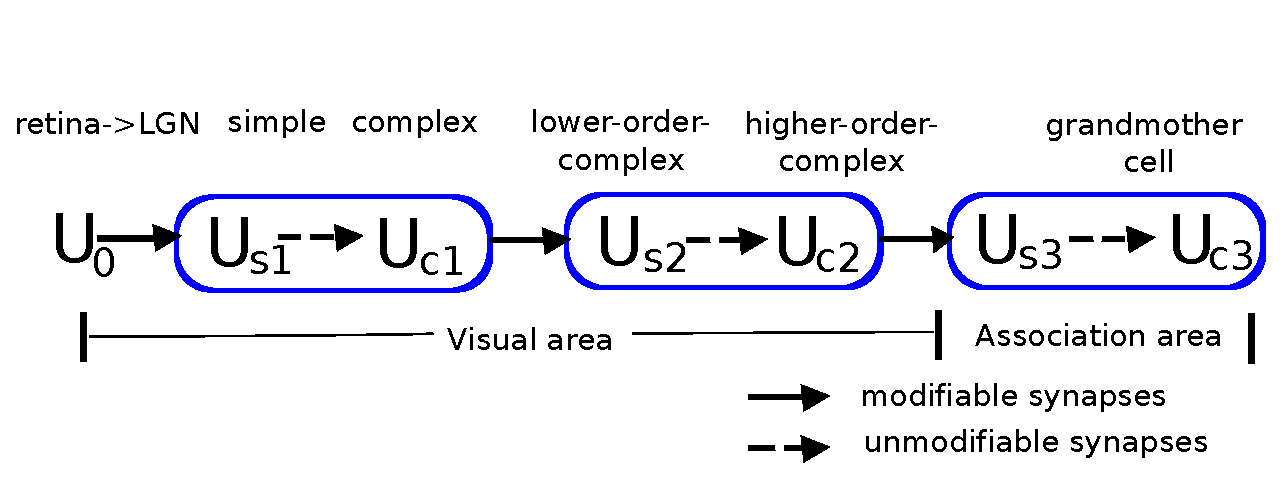
\includegraphics[width=8cm]{Figures/neocognitron.eps}
\caption{Neocognitron}
\label{neo}
\end{figure}
\section{Convolutional Networks}
\par Neocognitron was improved by  Yann LeCun \cite{lecun-86}, \cite{lecun-89e}, using backpropagation algorithm  to train the entire system. It uses local receptive fields, share weights and  sub-sampling to achieve  shift, position and distortion invariance. A typical Convolutional Network called  LeNet-5 was proposed by   Yann LeCun et al. \cite{LeCun1998}  for document recognition. Using \allowbreak local receptive fields, network can extract elementary visual features such as edges, end points and corners. These features will be combined to obtain high order features in the following layers. Elementary feature detectors with identical weights can be useful in different parts of the image. So the units with  the same set of weights are arranged in plane, and output from  the units of a plane is called  a feature map. Units in  a feature map perform the same operation on different parts of the same image. A convolution layer is composed of the set of feature maps with differently weighed units. In the implementation, a unit in the feature map scans the image and store the states in the feature map. This operation is equivalent to convolution with a kernel composed of a  set of weights and image. 

\par
A typical convolutional  network is composed of multiple stages with a filter bank layer, a non-linearity layer and a feature pooling layer \cite{lecun2010convolutional} followed by a classification network.\\
\begin{figure}[ht]

 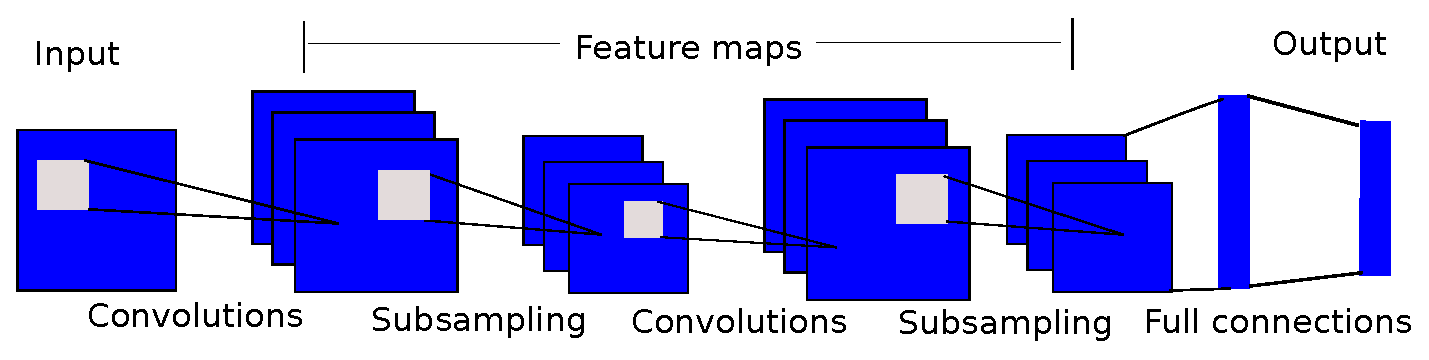
\includegraphics[width=8cm]{Figures/convent.eps}
\caption{A typical convolutional network architecture }
\label{net}
\end{figure}
\emph{Filter Bank Layer:} This layer computes $y_{j}$ the convolution between an input feature map   $x_i$ and trainable filter kernel $k_{ij}$ 
 ie. $y_j=b_j+\sum_i {k_{ij}*x_i}$, where $b_j$ is a trainable bias, $i$ and $j$ are  array indices, and $*$ is the convolution operator.\\
\emph{Non-Linearity Layer:} This layer applies a non-linearity function such as $tanh(x)$ or $(1+e^{-x})^{-1}$ to unit output. But to reduce training time with gradient descent, new implementations uses the function $max(0,x)$. Units with this non-linearity is called Rectified Linear Units (ReLUs) \cite{Nair2010}.\\
\emph{Feature Pooling Layer:} It  reduces the dimension of  feature map by applying the techniques like averaging or max-pooling.


% -------------------------------------------------------------------------

\begin{figure}[t]

\begin{minipage}[b]{.48\linewidth}
  \centering
  \centerline{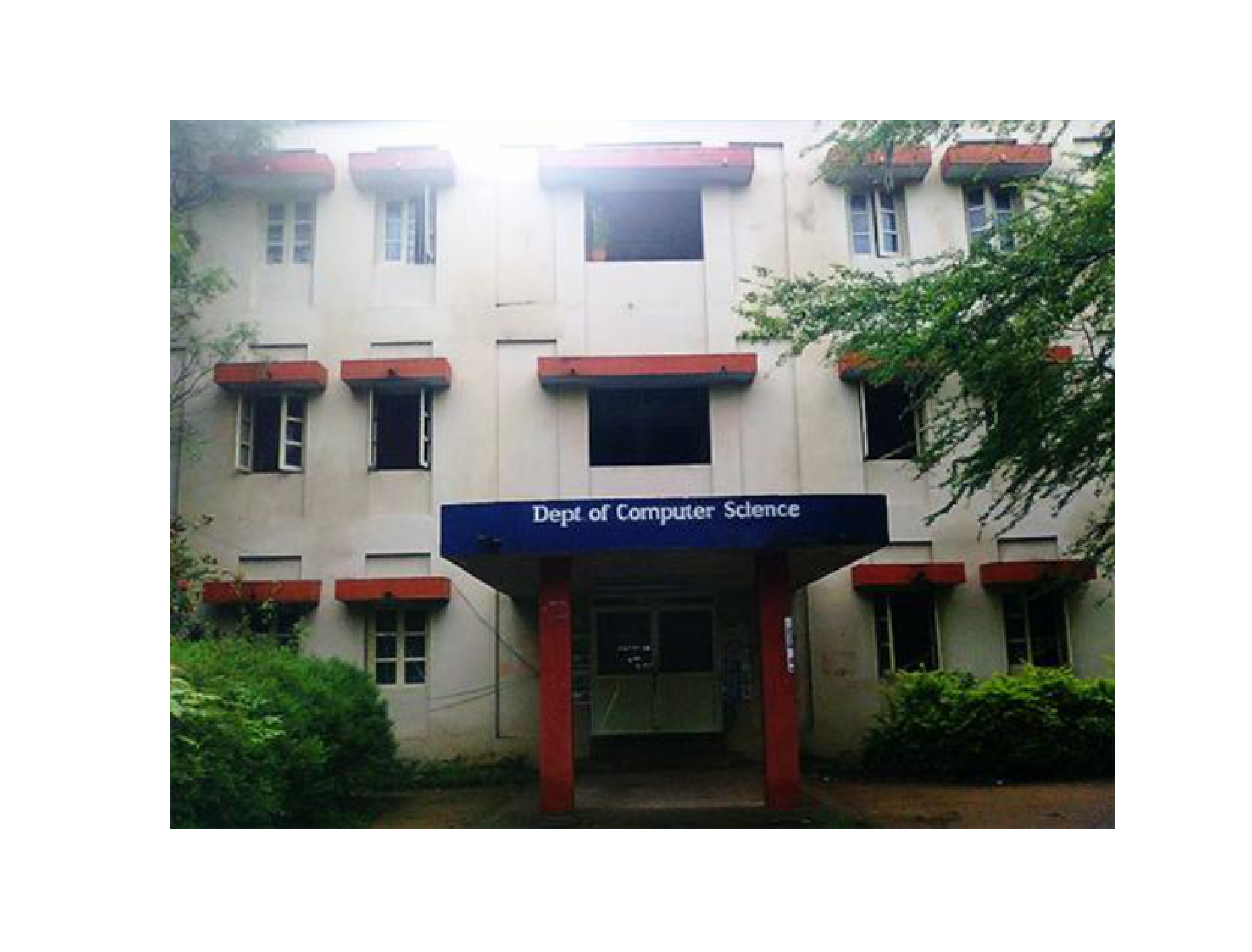
\includegraphics[width=4.0cm]{Figures/org}}
%  \vspace{2.0cm}
  \centerline{Input image}\medskip
\end{minipage}
%
\begin{minipage}[b]{.48\linewidth}
  \centering
  \centerline{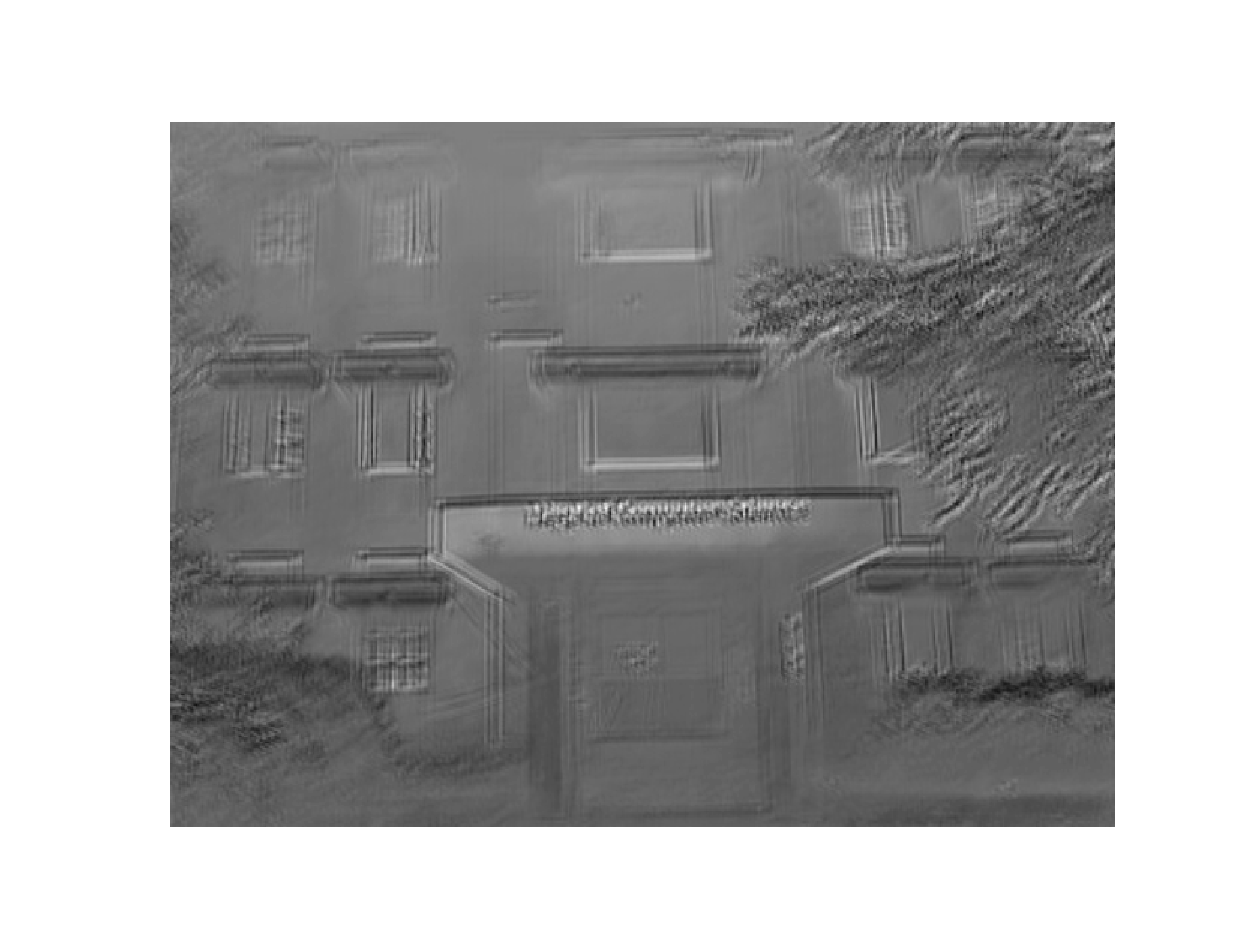
\includegraphics[width=4.0cm]{Figures/first}}
%  \vspace{1.5cm}
  \centerline{Output - first component }\medskip
\end{minipage}
\hfill
\begin{minipage}[b]{0.48\linewidth}
  \centering
  \centerline{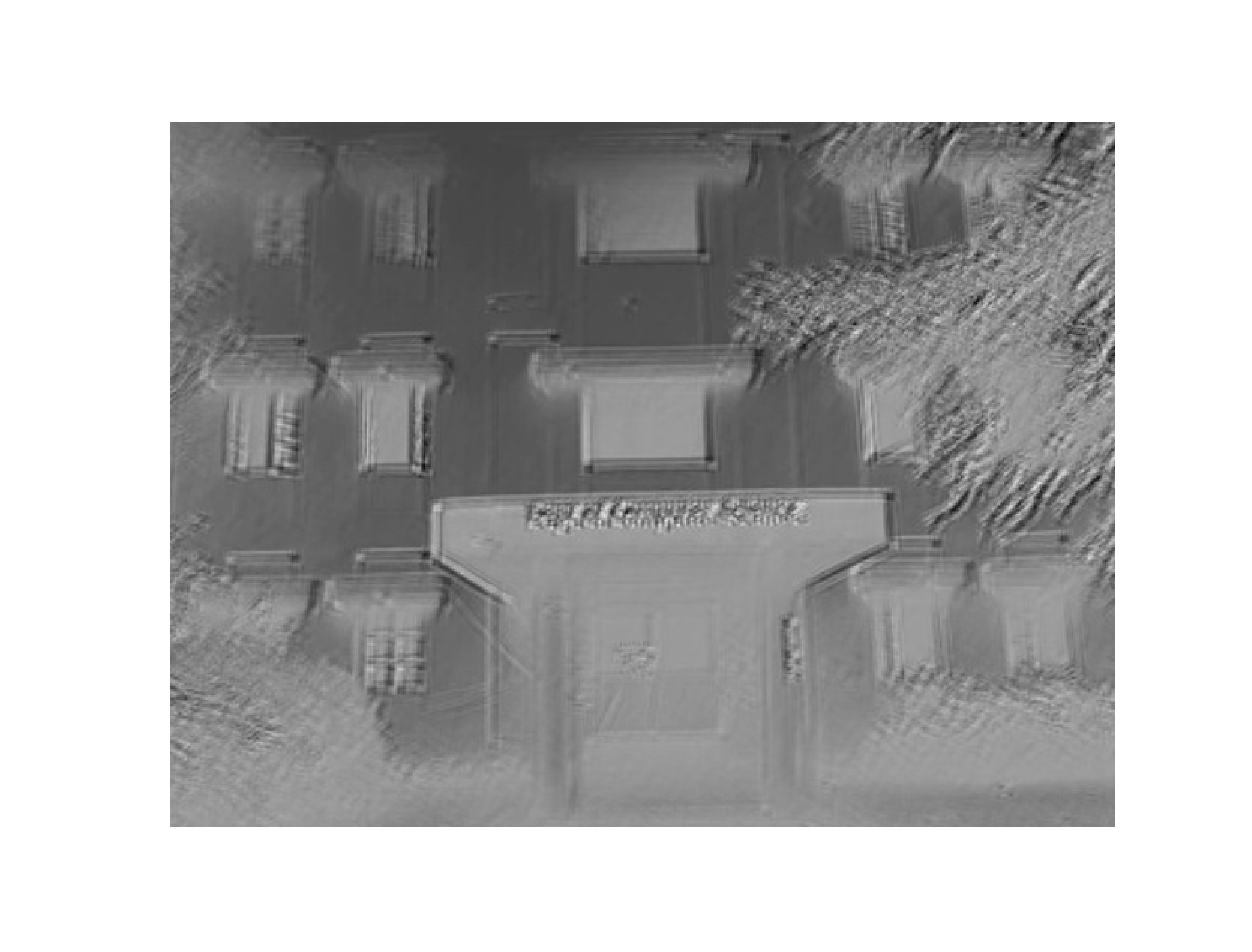
\includegraphics[width=4.0cm]{Figures/second}}
%  \vspace{1.5cm}
  \centerline{Output - second component}\medskip
\end{minipage}
%
\begin{minipage}[b]{0.48\linewidth}
  \centering
  \centerline{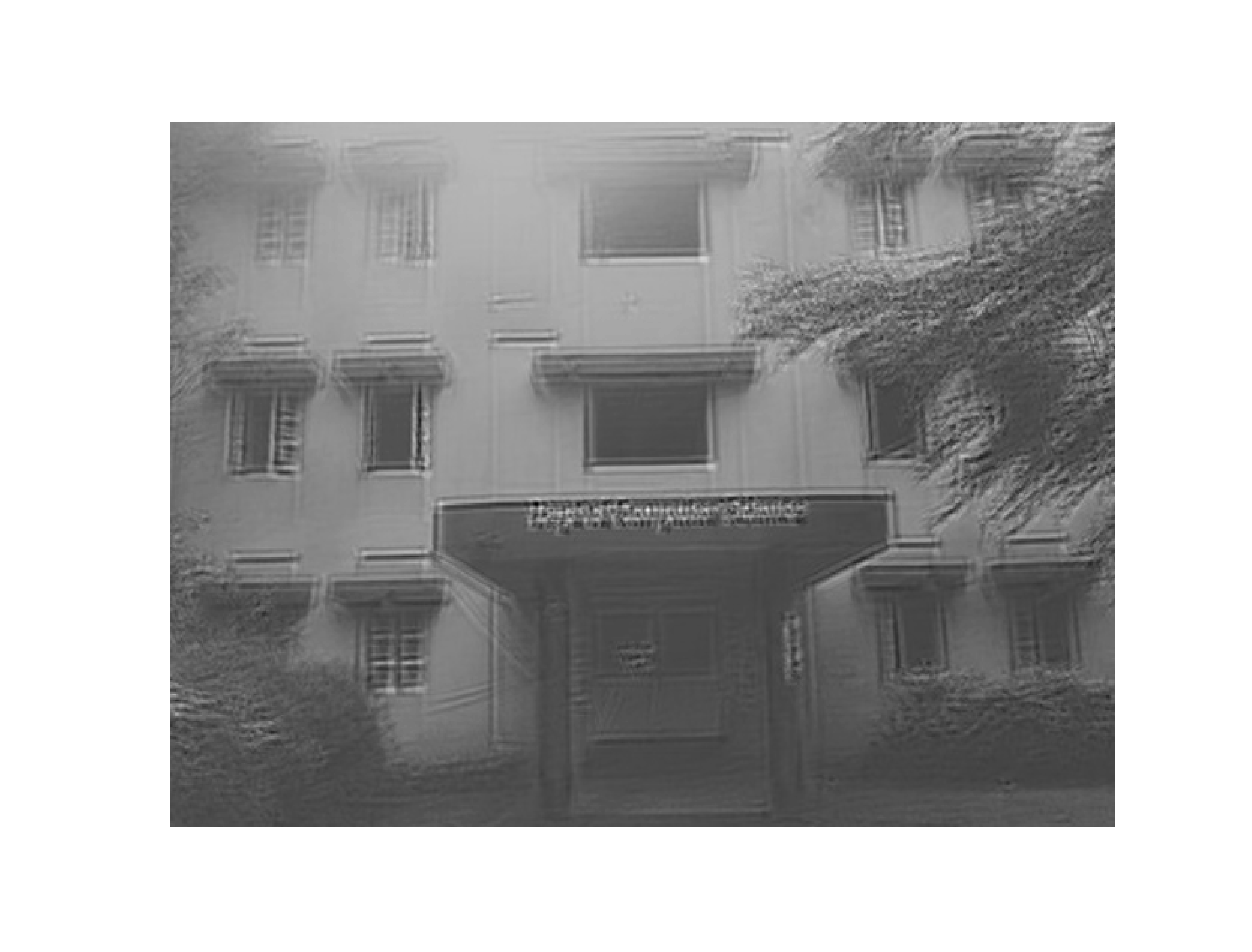
\includegraphics[width=4.0cm]{Figures/third}}
%  \vspace{1.5cm}
  \centerline{Output - third component}\medskip
\end{minipage}
%

\caption{Output of a randomly initialized convolution filter.
}
\label{fig:res}
%
\end{figure}




But this architecture was limited by the availability of computing power and  sample data sets. 
%2012

\section {Deep convolutional networks}
In the last few years, convolutional networks shows a significant performance improvement in many small scale image classification on data sets  such as MNIST \cite{Ciresan:2012g}, CIFAR-10, CIFAR-100, SVHN \cite{lee2014deeply}, and STL-10 \cite{deepfwd}. Krizhevsky, et al. \cite{Krizhevsky2012a} proposed a network  of 60 million parameters and 650,000 neurons, with five convolutional layers followed by max-pooling layers and three fully-connected layers. Data set used in this experiment was a subset of ImageNet dataset, used in the competition ImageNet Large-Scale Visual Recognition Challenge (ILSVRC) \cite{imagenet} and reported an error rate of 15.3\%. ILSVRC data set includes 1.2 million images that contain 1,000 categories. This network uses rectifier  as the function in neurons.  Even if it shows improvement in speed, this  ill-conditioned parameterization must be studied further to understand the effect in very large networks.


%2013

\subsection{Network in Network }
Inspired by the work of Ian J. Goodfellow et al..\cite{Goodfellow2013} on max out networks,  Min Lin et al. \cite{Lin2013} introduced a micro-network in each convolution layer so that it will compute more abstract features.This network gave a state-of-the-art performance in  ILSVRC 2013 competition with an error rate of 12.95\%.They used NVIDIA TITAN GPU to train the network. Using multilayer perceptron instead of voting to approximate convex functions of each  local patches may result in a good accuracy; but this is equivalent to moving linear separability problem into another hyperspace. So, if the input is in high frequency, this will end up in modeling large number of hidden layers and make the network structure more dependent on the problem. It will diverge the idea of the convolution network from \emph{learn anything} to a \emph{local search}.

\subsection{Visualizing Convolutional Networks}

Matthew D. Zeiler and Rob Fergus \cite{Zeiler2013} presented a method to visualize the function of intermediate feature layers of convolutional networks and used it as a diagnostic tool to improve  the model proposed by Krizhevsky et al. \cite{Krizhevsky2012a}. This method helped  them  to understand  the activation in the feature maps with respect to the input patterns. It shows that Krizhevsky et al.'s architecture does not have  enough mid frequency coverage in the first layer filters and causes aliasing artifacts by large stride in the first layer convolutions. Authors solved this problem by decreasing filter size to $7\times7$ and reducing stride to 2. This implementation won the  ILSVRC 2013 competition with an error rate of 11.74\%. These  techniques might be more useful if it can relate to any of the learning formulations instead of vague approximations of a non-invertible function.


%2014

\subsection{Spatial Pyramid Pooling in Deep Convolutional Networks}
Instead of using fixed input size in convolutional networks, Kaiming He et al. \cite{He2014} suggested  the use of a spooling strategy called  Spatial Pyramid Pooling (SPP) \cite{Grauman2005} \cite{1641019} to avoid cropping or warping of images. It introduced a new layer on top of the convolution layer and performed aggregation  based on Bag-of-Words (BoW) model. However, the classical backpropagation training methods expect layers to have a fixed   size.  This problem can be solved by using two fixed size networks with shared parameters and switch the network on alternate epochs. Network was trained using a single GeForce GTX Titan GPU with a starting  learning rate of 0.01 and achieved  a less  error rate of 8.06\% on  ILSVRC 2014 data set. 
\par 
This implementation improves the performance of baseline architectures including ZF-5 \cite{Zeiler2013}, Convnet \cite{Krizhevsky2012a} and Overfeat-5/7. Even if  the accuracy of convolutional networks will improve on multi-size training, multi-level pooling, and full-image representations, all these methods will increase both time and space complexity of the system.
%




\subsection{Going deeper with convolutions }
Christian Szegedy et al. \cite{Szegedy} proposed a network named GoogLeNet with receptive field (input layer) of size $244\times244$ with the number of layers around 100. Network is trained using asynchronous stochastic gradient descent with 0.9 momentum and fixed learning rate schedule based on the number of epochs. Learning procedure took advantage of  model and data-parallelism in a CPU-based cluster environment. This network gave an error rate of  6.67\%  on  ILSVRC 2014 data set. The experimental analysis shows that use of existing dense  blocks to  build the sparse structure can improve the  performance of convolutional networks. Even if higher depth will increase the accuracy, this system will end up with implementing large number of hidden layers to increase accuracy for a high frequency input. 


\section{VERY DEEP CONVOLUTIONAL NETWORKS }
Karen Simonyan and Andrew Zisserman \cite{Arge2015} evaluated the effect of network depth in image classification using very small convolution filters. Their deep network architecture comprised of fixed  size input layers, a stack of convolution layers, three Fully-Connected (FC) layers and  5 max-pooling layers for spatial pooling  over a $2 \times 2$ pixel window with stride 2. Hidden layers are modeled using Rectified Linear Units (ReLU) \cite{Nair2010}. On the hardware side, it uses a multi-GPU system with NVIDIA Titan Black GPUs. Network is trained using multinomial logistic regression  based on backpropagation with momentum of 0.9 and  batch size  256.
\par
It has been observed that greater depth with small convolution filters and  initialization of certain layers will cause the learning process to converge in less number of epochs and gain significant improvement in accuracy. This model of the convolution network does not differ from the classical architecture proposed by LeCun et al. \cite{LeCun1998}. This implementation results in a significant improvement in accuracy with  an error rate of 6.8\% in ILSVRC 2014 of ImageNet.

\begin{subsection}{Scaling up Image Classification}
The latest attempt in image classification with an error rate of 5.98\% in ImageNet data set is reported by Ren Wu et al. \cite{Wu2015} of Baidu research. They developed an end to end deep learning  system named Deep Image. It uses a highly optimized parallel algorithm to implement large deep neural network with augmented input data. The network is trained using Stochastic Gradient Descent algorithms (SGD) on a custom built high performance system comprised of 36 server nodes, each with 2 six-core Intel Xeon E5-2620 processors and 4 NVIDIA Tesla K40m GPUs. System  uses an InfiniBand  network for interconnections. Parallelism strategies used in this network are model-data parallelism and data parallelism. These methods have been proposed by Alex Krizhevsky \cite{Krizhevsky2014} and Omry Yadan et al. \cite{Yadan2013} for training convolutional neural networks with SGD on a  multiple GPU systems. However, it is not easy to extend the same strategies to multiple GPU clusters because of the communication overhead. The major objective is to minimize network data transfers and dynamic computation. So it uses butterfly synchronization and lazy update strategies to achieve data parallelism in the gradient computation. These approaches shows that model-data parallelism is better when number of GPUs is less than 16. Implementation of Data parallelism in a large number of GPU cluster is better because of the constant communication requirements.
\par
Data augmentation techniques are used to increase the number of labeled images in the training set. This includes color casting, vignetting, lens distortion, rotation, flipping and cropping. But this data augmentation techniques does not solve the major problems such as occlusion, presence or absence of structural components, and lighting conditions.
\begin{table*}[ht]
\captionsetup{justification=centering,belowskip=-2pt,aboveskip=-2pt}
\caption[]{ Comparative analysis of state-of-the-art deep convolutional network based image classification algorithms using ILSVRC dataset.}
 \begin{tabular}{ | p{2.7cm} | l | p{1.4cm} |p{1.3cm} |p{.8cm} |p{1.3cm} |p{1.1cm} |p{5cm}|}

    \hline
\textbf{Team}	&\textbf{Year}	&\textbf{Data Augmentation}	&\textbf{Scalable over network}	&\textbf{Time taken}	&\textbf{Hardware}	&\textbf{Error rate} &\textbf{Observations}
\\ 
\hline
Ren Wu et al. \cite{Wu2015}&2015&Aggressive&Yes&8.8 hours&Multi-GPU Cluster&5.98\%&Aggressive augmentation  will make the problem dependent on data set.\\
\hline
Karen Simonyan et al. \cite{Arge2015}&2014&Minimum&No&3 weeks&Multi-GPU&6.80\% &Effect of small convolution filter in low frequency domain need to be studied.\\
\hline
Christian Szegedy et al. \cite{Szegedy}&2014&Minimum&Yes&1 week&CPU Cluster&6.67\% &Inserting more layers will make system depend on the data set.\\
\hline
Kaiming He et al. \cite{He2014}&2014&Minimum&No&4 weeks	&Single GPU	&8.06\% &Good method, but higher time complexity.\\
\hline
Matthew D. Zeiler et al. \cite{Zeiler2013}&2013&Minimum&No&12 days&Single GPU&11.74\% & Visualizations are not possible in very deep network.\\
\hline
Min Lin et al. \cite{Lin2013}&2013&Minimum&No&12 days&Single GPU&12.95\% &Inserting more layers will over-fit the system.\\
\hline
Krizhevsky, et al.\cite{Krizhevsky2012a}&2012&Minimum&No&6 days	&Multi-GPU&15.30\%&Effect of rectifier must be studied further.\\
\hline

\end{tabular}
\label{table_cp}
\end{table*}
\par
 Major contribution of this work is the demonstration of tremendous computational power required to  achieve high accuracy in image classification.
It also shows that augmented multi-scale images can be combined to achieve less error rate in convolutional network in the context of the image classification. 
 \end{subsection}
 \section {Observations}
In recent years, the research community has reported several image classification algorithms based on deep convolutional network which gives less rate. A comparative analysis of recent futuristic deep convolutional networks is shown in Table \ref{table_cp}.
  Ren Wu et al. \cite{Wu2015} uses aggressive data argumentation and high computational power to reduce the computational time and error rate. Karen Simonyan et al. \cite{Arge2015} work shows, error rate can be reduced using small convolution filters. Christian Szegedy  et al. \cite{Szegedy} and Min Lin et al. \cite{Lin2013} introduces a set of hidden layers to model local patches. Kaiming He et al. \cite{He2014} uses a different pooling technique to reduce the error rate. Krizhevsky, et al. \cite{Krizhevsky2012a}  introduces  rectifier  as the neuron function. Although significant progress has been made in the last few years, there is still room for further research and improvement. Major observations from our study are listed below.
 \begin{itemize}
 \itemsep0pt 
 \item  Wisely chosen data  augmentation techniques can increase the performance of the network. But need to be tested with multiple data set.
 \item Data parallelism and model parallelism can increase the speed of the training process. This area can be exploited further to increase the speed of the training process.
 \item Greater depth with small convolution filters will improve the accuracy. But, response to different frequency input must be studied.
 \item Performance of the network will get improved if images at difference scales are used for training.
 \item Use of different pooling technique such as spatial pyramid pooling in sub-architectural level may reduce the error rate. 
\end{itemize}
\section{conclusion}
This paper attempts to provide a  review of research on deep convolutional networks  and provide an overview of  its architecture and performance. Majority of the reviewed  works are reported from ImageNet Large-Scale Visual Recognition Challenge. These networks can only be trained using very expensive computing resources such as multiGPU cluster  to achieve more accuracy on large data sets. So  this research heavily depends on other research domains such as parallel algorithms, computer networks and multicore architecture. Because of the heavy computational requirements, it is not easy to apply this method directly  to the small level computing platforms such as embedded systems and application level  processors. On the other side, these methods can easily bring  live with the help of  cloud computing infrastructure, so to the mobility solutions such as mobile phones and the web.

\bibliographystyle{IEEEbib}
\bibliography{refs}

\end{document}
